% !TeX encoding = UTF-8
\section{Traumap{\"a}dagogik - Haltung, Konzepte, traumasensible Organisationsentwicklung}

Traumapädagogik charakterisiert sich durch eine Grundhaltung, die als Basis des pädagogi-schen Handelns zu verstehen ist und sich in einem wertschätzenden pädagogischen Verständ-nis des Kindes zeigt (vgl. Schmied \& Lang 2012: 339). Aus den verschiedenen pädagogischen Konzepten, die zunächst aus der Praxis heraus entstanden sind, lassen sich handlungsleitende Inhalte herausarbeiten (vgl. Rothdeutsch-Granzer u. a. 2015: 178 f.). Traumapädagogik als konsequente Anwendung des psychotraumatologischen Wissens in der Ausgestaltung des pädagogischen Alltags und ein wertschätzendes Verständnis der betreuten Menschen berück-sichtigt alle Ebenen einer Organisation (vgl. Schmid \& Lang 2012: 339 ff.; BAG-TP 2011: 5) und kann als ein traumasensibler Organisationsentwicklungsprozess verstanden werden. Im Folgenden werden die traumapädagogische Haltung (2.1), wichtigste traumapädagische Kon-zepte und deren Inhalte (2.2) sowie die Traumap{\"a}dagogik als ein pädagogischs Konzept (3.3) fokussiert.

\subsection{Traumapädagogische Haltung}

Eine traumasensible Grundhaltung stellt die Basis für die Entwicklung traumapädagogischer Konzepte sowie eine Orientierung für das praktische und pädagogische Handeln dar (vgl. BAG-TP 2011: 4). Dabei soll das Wissen um die möglichen Folgen belastender Erlebnisse berücksichtigt werden, und es sollen die Ressourcen der Kinder und Jugendlichen im Mittel-punkt stehen (vgl. ebd.). Für die Entstehung der Traumap{\"a}dagogik seien Psychotraumatologie ebenso wie Soziale Arbeit, bindungstheoretische Grundlagen und Resilienzforschung, Neuro-

biologie und die therapeutischen Wissenschaften von Bedeutung (vgl. Weiß 2016b: 22). Traumap{\"a}dagogik beziehe sich auf Reformpädagogik, emanzipatorische Pädagogik und ver-trete das in der humanistischen Pädagogik und Psychologie begründete Menschenbild (vgl. Weiß 2016b: 23). Auf dieser Basis ist eine Reihe von Konzepten entstanden, die sich zwar in Inhalten und Gewichtung im pädagogischen Handeln unterscheiden, allerdings eine gemein-same Grundhaltung haben (vgl. ebd.). Die traumapädagogischen Standards formulieren dazu folgende fünf Handlungsansätze (vgl. BAG-TP 2011: 5 ff.):

\begin{itemize}[noitemsep]
\item „Die Annahme des guten Grundes – Alles was ein Mensch zeigt, macht Sinn in seiner Geschichte!“ (ebd.: 5) 
\item „Wertsch{\"a}tzung – Es ist gut so, wie du bist!“ (ebd.: 5) 
\item „Partizipation – Ich traue dir was zu und {\"u}berfordere dich nicht!“ (ebd.: 6) 
\item „Transparenz – Jeder hat jederzeit ein Recht auf Klarheit!“ (ebd.: 6) 
\item „Spaß und Freude – Viel Freude tr{\"a}gt viel Belastung“ (ebd.: 7)
\end{itemize}

Im Zentrum der traumapädagogischen Haltung steht die Annahme des guten Grundes (vgl. Weiß 2016b: 23; Rothdeutsch-Granzer u. a. 2015: 177). Das Verhalten des Kindes wird dabei im Kontext seiner Biografie und Entwicklung als normale Reaktion auf eine außerordentliche Belastung verstanden. Das Kind soll in seinem Wesen und samt seinen Schwierigkeiten, die als Überlebensstrategien zu verstehen sind, angenommen und wertgeschätzt werden (vgl. ebd.). Transparenz im pädagogischen Alltag und die Teilhabe an der Gestaltung der eigenen Lebensbedingungen ermöglichen Kindern und Jugendlichen, Autonomie, Kompetenz und Zugeh{\"o}rigkeit zu erleben (vgl. BAG-TP 2011: 6). Dies sind wichtige Faktoren, die die seelische Gesundheit beeinflussen und eine Alternative zu den vorangegangenen Erfahrungen wie Gewalt, Vernachl{\"a}ssigung und/oder Missbrauch anbieten. Spaß und Freude zu erleben, wirkt ausgleichend zu den belastenden Erlebnissen, die die Gefühlswelt in ein Ungleichgewicht bringen (vgl. ebd.). Die traumapädagogische Haltung solle nicht nur den Kindern und Jugendlichen gegenüber gelten, sondern die MitarbeiterInnen und KooperationspartnerInnen miteinschließen (vgl. Schmid \& Lang 2012: 345).

\subsection{Traumapädagogische Konzepte – handlungsleitende Inhalte}
Traumapädagogik als Sammlung von Konzepten, die traumatisierte Mädchen und Jungen sowie junge Erwachsene im pädagogischen Alltag unterstützen, ist aus der pädagogischen Praxis entstanden. Diese Konzepte weisen einige Gemeinsamkeiten auf, vor allem in Bezug auf die Grundhaltung (siehe 2.1), als auch Unterschiede in Inhalten und im Handeln (vgl. Weiß 2016b: 23). Aus diesen Konzepten lassen sich handlungsleitende Inhalte für das pädagogische Handeln herausarbeiten (vgl. Rothdeutsch-Granzer u.a., 2015: 178 f.; siehe Abbildung \ref{fig:inhalte})

\begin{figure}[h]
  \centering
  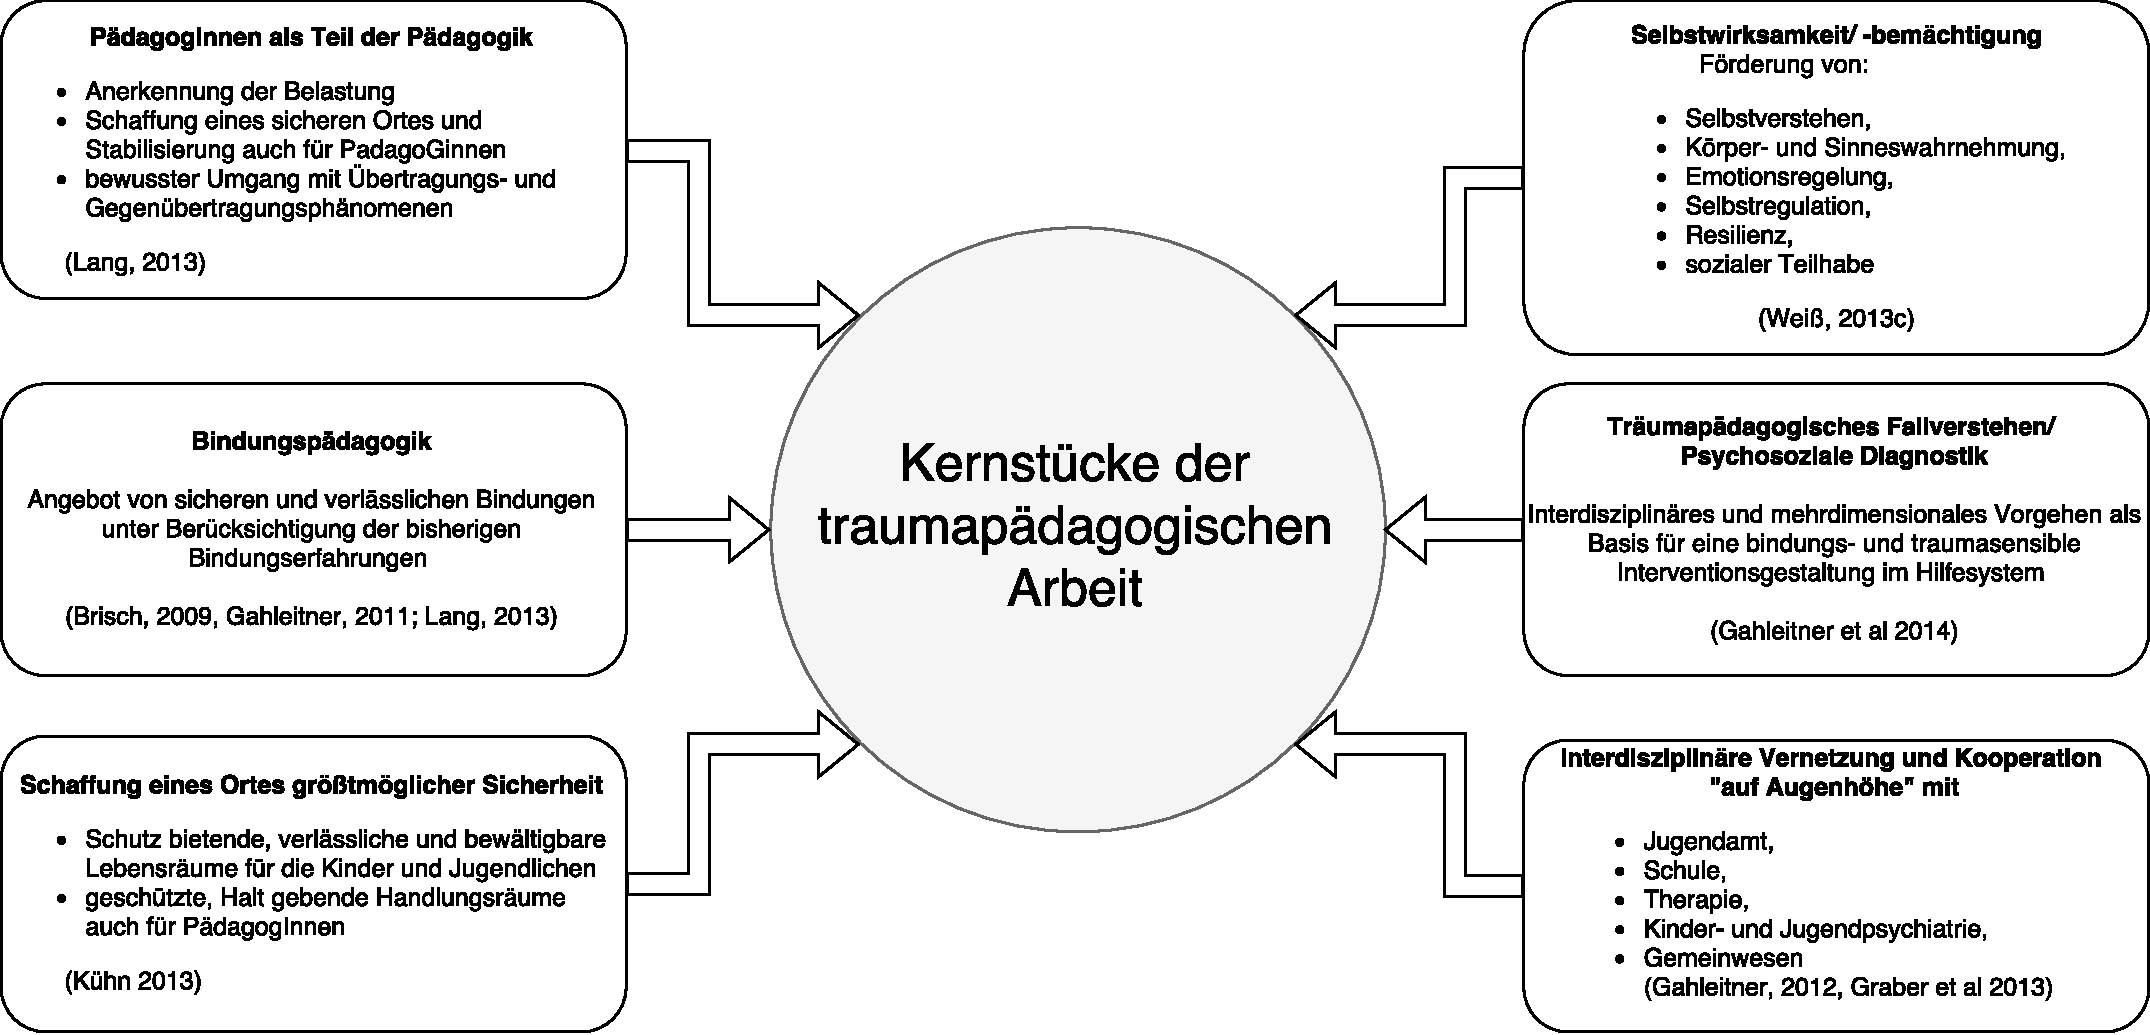
\includegraphics[scale=0.45]{abbildung2}
  \caption
      [Handlungsleitende Inhalte der traumapädagogischen Arbeit]
      {Handlungsleitende Inhalte der traumapädagogischen Arbeit (nach Rothdeutsch-Granzer u.a., 2015: 179)}
  \label{fig:inhalte}
\end{figure}

Kühn (2014: 21) bezeichnet drei Kernkonzepte als richtungsweisend in der Traumap{\"a}dagogik: \textit{Pädagogik des sicheren Ortes} (vgl. Kühn 2006), \textit{Traumazentrierte Pädagogik} nach Uttendörfer (2008) und \textit{Pädagogik der Selbstbemächtigung} nach Weiß (2016a). Mittlerweile sind weitere Konzepte und Anwendungen entstanden, die die Vielfältigkeit der Handlungsfelder zeigen, in denen psychotraumatologisches Wissen gefragt ist. Das sind, um einige Beispiele zu nennen: \textit{Traumapädagogische Gruppenarbeit} nach Bausum (2013), \textit{Stabilisierung und (Selbst-)Fürsorge für PädagogInnen} (Lang 2013), \textit{Traumapädagogik in der Schule} (Ding 2013, Zimmerman 2016) und \textit{Milieutherapeutische Konzepte} (Gahleitner 2011). Auch in weiteren Handlungsfeldern und für AdressatInnen wie z. B. Ehe- und Familienberatung, Gefangenenseelsorge, Gewaltprävention, Frauenhäuser, Wohneinrichtungen für unbegleitete minderjährige Flüchtlinge etc. sei traumapädagogisches Wissen gefragt (vgl. Hantke 2015: 118).  

Die gemeinsamen Inhalte der Konzepte sind in Bezug auf den \textit{sicheren Ort} und die Bedeutung der Bindung sowie positiver Beziehungserfahrungen für die Traumabearbeitung am weitesten entwickelt (vgl. Weiß 2016b: 27). Viele Konzepte adaptieren (psycho-)therapeutische Methoden, um z. B. mit Fertigkeitstrainings oder Notfallkoffern die Emotionsregulation zu begleiten (vgl. ebd.: 28). Einige Konzepte betonen die Wichtigkeit und Bedeutung der traumatischen Übertragungs- und Gegenübertragungsreaktionen (vgl. Kessler 2016: 123 ff.; Schmid 2013: 48) und formulieren entsprechende Interventionen. Die Traumabearbeitung als ein Prozess der Selbstbemächtigung nach Weiß (2016b: 20) beinhaltet unter anderem: traumabedingte Einstellungen und Überzeugungen zu verändern; das Geschehen in die eigene Lebensgeschichte einzuordnen; die Möglichkeit, in der Gegenwart Sinn zu finden; Körperfürsorge und Körpergewahrsein zu entwickeln; Selbstregulation zu erlernen; die traumatischen Erinnerungen und den traumatischen Stress zu kontrollieren sowie soziale Teilhabe zu ermöglichen. Dieses Konzept betont vor allem die Expertenschaft der Kinder und Jugendlichen. Ihnen soll das Wissen über Traumatisierung zur Verfügung gestellt werden (vgl. ebd.).  

Schmid und Lang (2012: 347) sehen Psychoedukation als bedeutenden Bestandteil der Traumap{\"a}dagogik. Ziel sei es, den Kindern und Jugendlichen ihre Reaktionen und Symptome, neurobiologische Abl{\"a}ufe, das Entstehen von Spannungszust{\"a}nden, K{\"o}rperreaktionen und Dissoziationen etc. in einer altersangemmessenen und verständlichen Form mit bildhafter Sprache und grafischer Unterstützung zu erklären. Dabei sei die Botschaft wichtig, dass Symptome und Schwierigkeiten der Heranwachsenden eine normale, menschliche Reaktion auf v{\"o}llig unnormale und unmenschlichet Erlebnisse darstellen. Wichtig sei es, dass das Kind und die mit ihm arbeitenden Erwachsenen die gleiche Terminologie benutzten, um eine gemeinsame Sprache für spätere Interventionen und Analyse von schwierigen Situationen zu entwickeln (vgl. Schmid \& Lang 2012: 347).

\subsection{Traumapädagogik als Konzept}
Die BAG-TP sieht die Notwendigkeit, die Erkenntnisse der Psychotraumatologie und der Hirnforschung in den Institutionen, in denen traumatisierte Mädchen und Jungen betreut werden, umzusetzen (vgl. BAG-TP 2011: 4 f.). Klare Haltungen, F{\"o}rderans{\"a}tze und Methoden, die in der Umsetzung traumap{\"a}dagogischer Konzepte unerl{\"a}sslich seien, bilden die Grundlage f{\"u}r die von der BAG-TP formulierten Standards zur traumap{\"a}dagogischen Arbeit in Einrichtungen der station{\"a}ren Kinder- und Jugendhilfe. Im Mittelpunkt eines traumapädagogischen Konzepts steht laut der BAG-TP, verlässliche Beziehungen im Alltag aufzubauen und zu gewährleisten, die Traumatisierten sozial und emotional zu stabilisieren sowie das Selbstvertrauen der zu betreuenden Kindern und Jugendlichen aufzubauen und zu stärken (vgl. ebd.). Dabei soll die traumapädagogische Grundhaltung (siehe 2.1) als Voraussetzung institutionell durchg{\"a}ngig erkennbar bleiben (vgl. BAG-TP 2011: 5 ff.). Eine Einrichtung, die traumapädagogisch arbeitet, soll zu einem sicheren Ort werden, an dem betroffene Kinder und Jugendliche „neue, erg{\"a}nzende Erfahrungen machen k{\"o}nnen, sich selbst und ihre Handlungsstrategien verstehen lernen, Entwicklungshemmnisse aufholen und sichere Bindungserfahrungen machen k{\"o}nnen“ (BAG-TP 2011: 4). Die Entwicklung dieses Ortes soll alle Beteiligten mit einbeziehen und als ein institutioneller und kontinuierlicher Prozess verstanden werden. Die Einführung eines traumapädagogischen Konzepts im Sinne eines sicheren Ortes soll mehrere Ebenen einer Institution miteinschließen (vgl. ebd.). Schmid (2013: 49) versteht das Einbeziehen der MitarbeiterInnen und der strukturellen Abläufe in die (trauma-)pädagogische Konzeption als zentral. Um den Kindern und Jugendlichen einen stabilisierenden, sicheren Rahmen zu bieten, bedarf es solcher MitarbeiterInnen und Strukturen, die selbst stabil und selbstwirksam sind. Die MitarbeiterInnen und Teams brauchen, um bei den Krisen stabilisierend zu wirken, dieselben Fertigkeiten wie die Kinder und Jugendlichen selbst (vgl. ebd.). Schmid (2013: 49) beschreibt eine Institution, die ein traumapädagogisches Konzept umsetzt, als eine Versorgungskette, am Anfang derer das Kind steht, das im Alltag unterstützt werden soll (siehe Abbildung \ref{fig:konzept}). Hierzu bedarf es jedoch stabiler und stabilisierender Strukturen auf allen Ebenen der Organisation (vgl. ebd.).

\begin{figure}[h]
  \centering
  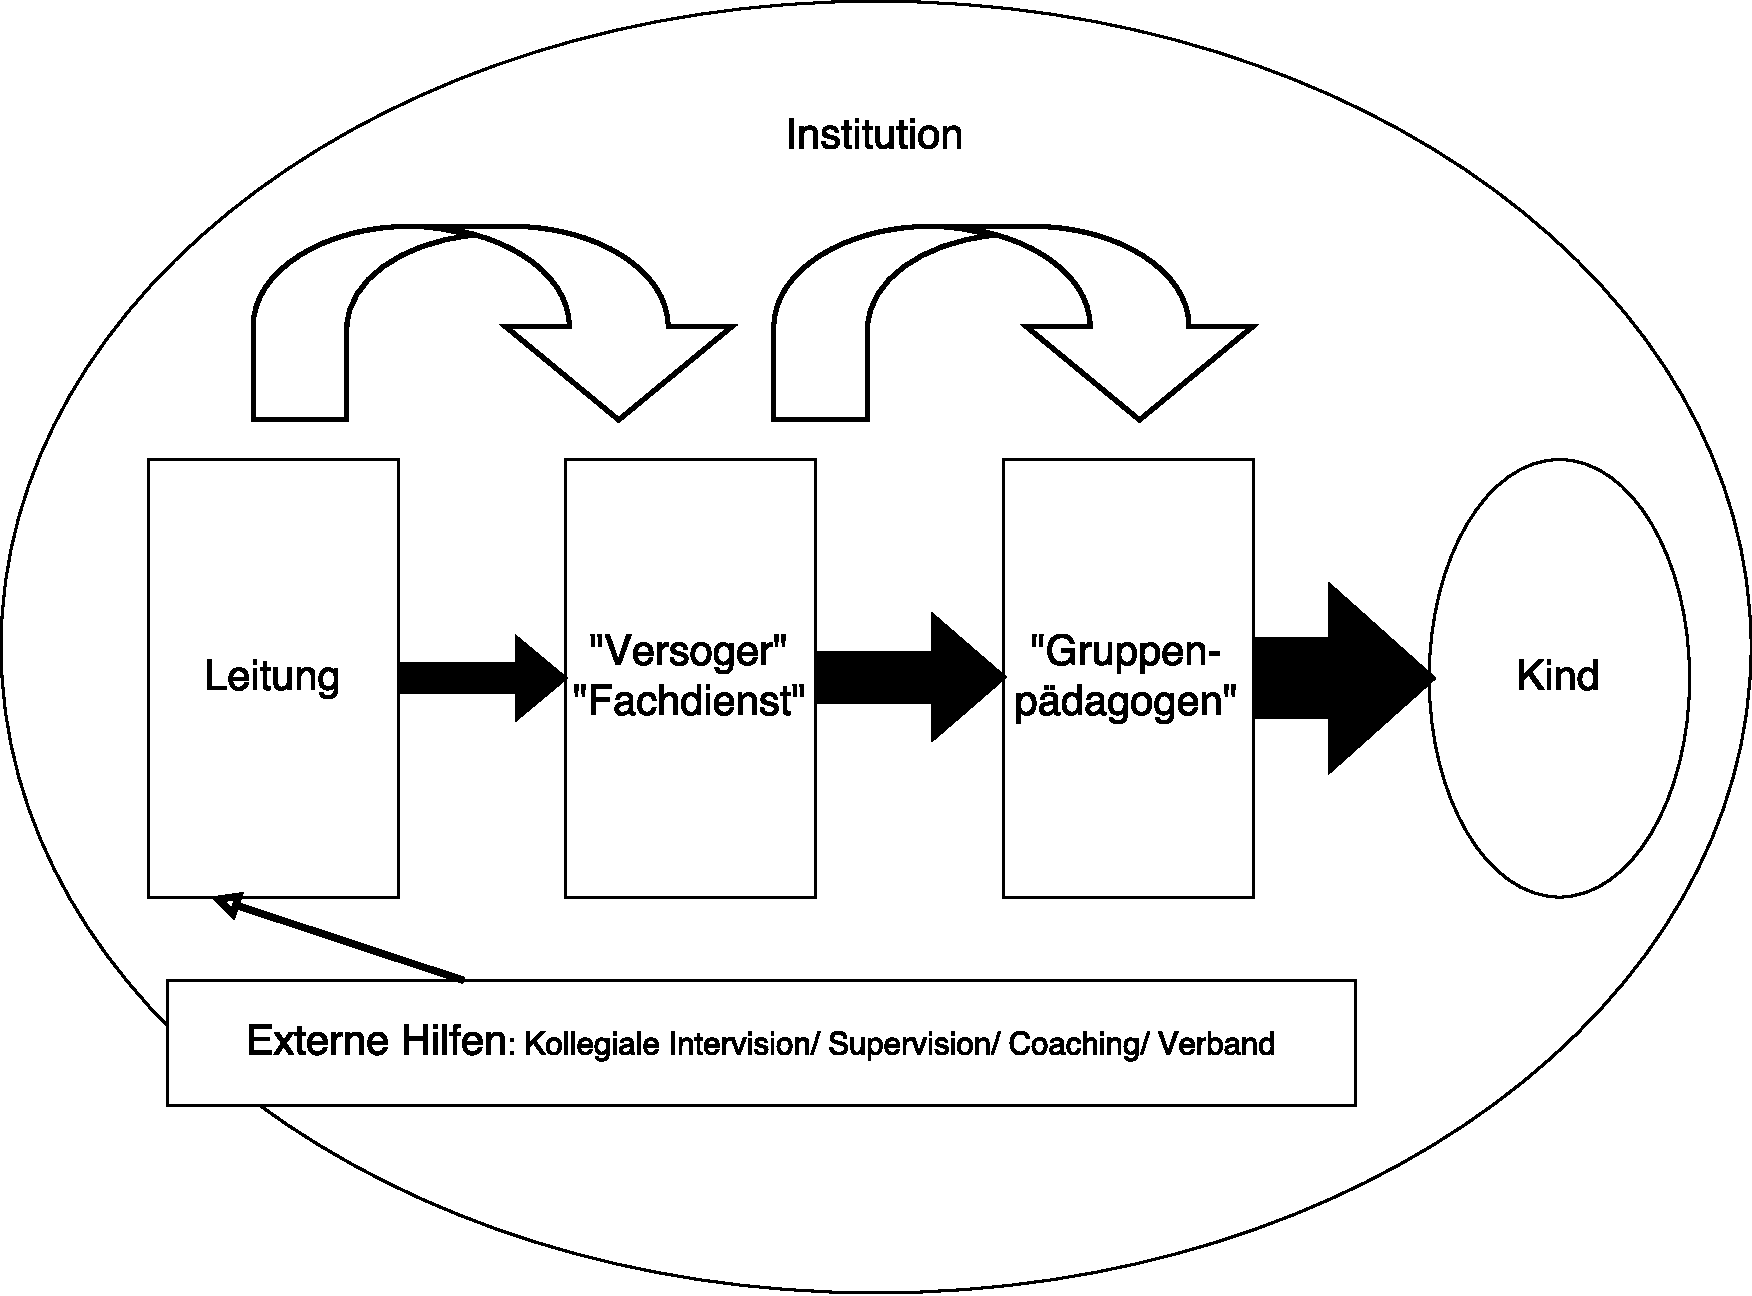
\includegraphics[scale=0.3]{abbildung3}
  \caption
      [Konzept einer Versorgungskette]
      {Konzept einer Versorgungskette (nach Schmid 2013: 49)}
  \label{fig:konzept}
\end{figure}

Traumap{\"a}dagogik sowie traumapädagogische Standards können laut Schirmer (2016: 443 f.) als Paradigmenwechsel in der Heimerziehung gewertet werden. Dieser besteht darin, dass die pädagogischen Fachkräfte, Kinder und Jugendlichen und die institutionellen Strukturen in das pädagogische Konzept im Sinne einer wertgeleiteten Organisations- und Personalentwicklung mit der zugrunde liegenden wertschätzenden verstehender Grundhaltung einbezogen werden. Diese Haltung richtet sich darauf, das „unerwünschte“ Verhalten reflexiv zu verstehen und gemeinsam nach Lösungen und pädagogisch nachvollziehbaren pädagogischen Interventionen zu suchen (vgl. ebd.).
